\chapter{数据获取与预处理}
本章将从系统使用的数据集,情感词典和预处理流程三方面进行介绍。
\section{数据集}
为了评估数据模型的准确性以及训练模型以便展示等目的,本文针对语句级和情感级两个任务获取了以下数据集。
\subsection{语句级数据集}
\begin{center}
\begin{longtabu} to 0.8\textwidth{X|X[3]}
\hline
名称 & 手机评论数据集\\
\hline
数据总数 & 2700条\\
语言 & 中文\\
比例 & 正向:负向=1700:1000\\
词数最大值 & 300词数量级\\
90\%词数 & 50词数量级\\
情感分类准确度 & 较为正确\\
语句特点 & 语句较为规范,感情较为强烈\\
获取方式 & 实验室内部资源\\
主要用途 & 初期评估模型可行性及模型展示\\
词频统计 & 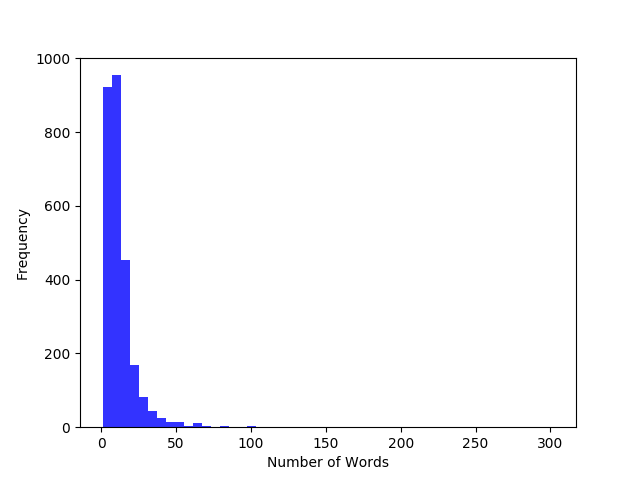
\includegraphics[width=0.6\textwidth, height=0.3\textwidth]{graphic/wordsnum_mobile.png}\\
\hline
%\caption{Mobile Dataset Word Number}
名称 & NLPCC 2014 SCDL数据集\\
\hline
数据总数 & 中文12500条,英文12485条,共24985条\\
官方测试集数据总数 & 中文2500条,英文2500条\\
语言 & 中文,英文\\
比例 & 中文 正向:负向=1700:1000\\
测试集比例 & 中文 正向:负向=1250:1250 英文 正向:负向=1250:1250\\
词数最大值 & 1000词数量级\\
90\%词数 & 200词数量级\\
情感分类准确度 & 不够准确\\
语句特点 & 语句较为口语化,有广告等中性语句\\
获取方式 & \url{http://tcci.ccf.org.cn/conference/2014/pages/page04_sam.html}(Accessed at: 5/21/2017)\\
主要用途 & 评估模型性能\\
词频统计 & 
中文\newline
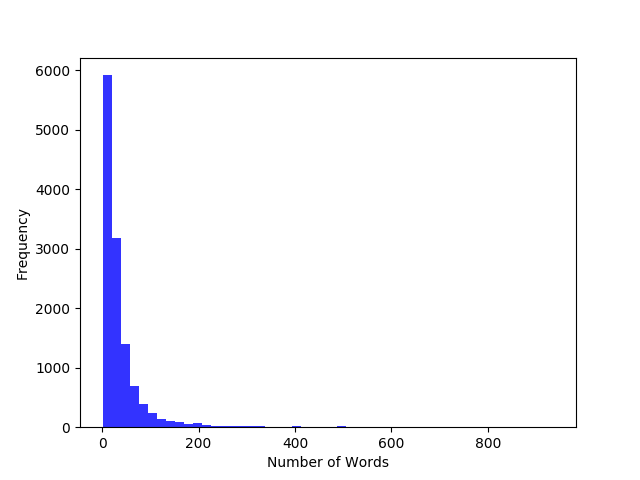
\includegraphics[width=0.6\textwidth, height=0.3\textwidth]{graphic/wordsnum_nlpcc_zh.png}
英文
\newline
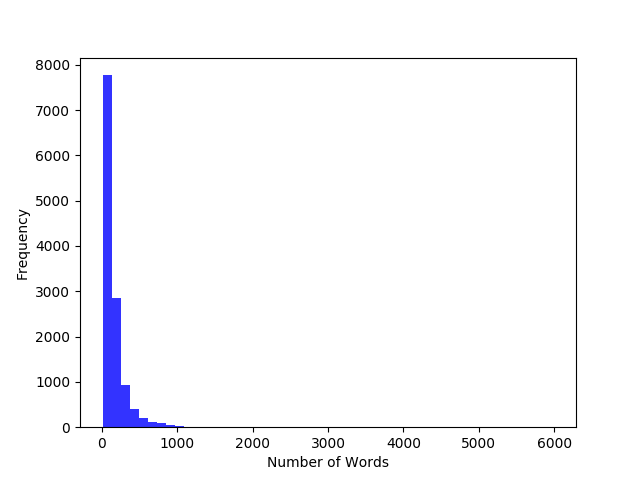
\includegraphics[width=0.6\textwidth, height=0.3\textwidth]{graphic/wordsnum_nlpcc_en.png}\\
\hline
名称 & 携程数据集\\
\hline
数据总数 & 250463条\\
语言 & 中文\\
比例 & 正向:负向=193138:57325\\
词数最大值 & 1750词数量级\\
90\%词数 & 250词数量级\\
情感分类准确度 & 不够准确\\
语句特点 & 语句较为口语化\\
获取方式 & 通过selenium模拟浏览器爬取到388067条带评分的携程酒店评论,其中评分小于4.0的定为负向,评分等于5的定为正向\\
主要用途 & 模型展示及标注实体数据集\\
词频统计 & 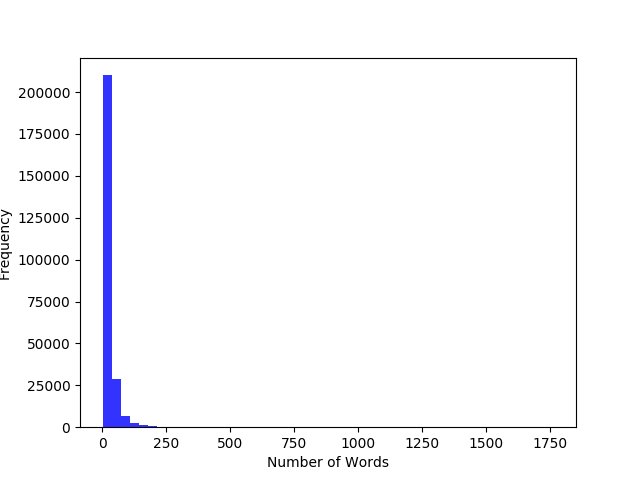
\includegraphics[width=0.6\textwidth, height=0.3\textwidth]{graphic/wordsnum_xiecheng.png}\\
\hline
\end{longtabu}
\end{center}  
\subsection{实体级数据集}
\begin{center}  
\begin{longtabu} to 0.8\textwidth{X|X[3]} 

\hline
名称 & SemEval2014Task4数据集\\
\hline
数据总数 & Laptop子数据集为3045条,Restaurants子数据集为3041条\\
语言 & 英文\\
词数最大值 & 80词数量级\\
90\%词数 & 50词数量级\\
情感分类准确度 & 较为正确\\
语句特点 & 语句较为规范,感情较为强烈\\
获取方式 & \url{http://alt.qcri.org/semeval2014/task4/}(Accessed at: 5/21/2017),取其中已标注的训练数据部分\\
主要用途 & 评估模型可行性及模型展示\\
词频统计 & 
Laptop\newline
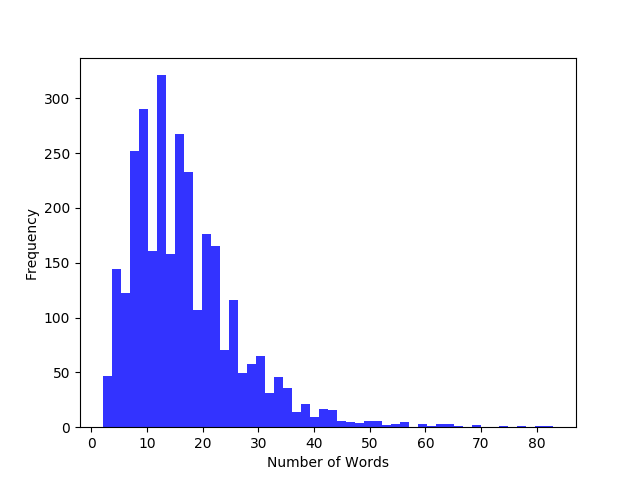
\includegraphics[width=0.6\textwidth, height=0.3\textwidth]{graphic/wordsnum_semval14_laptop.png}
\newline
Restaurant
\newline
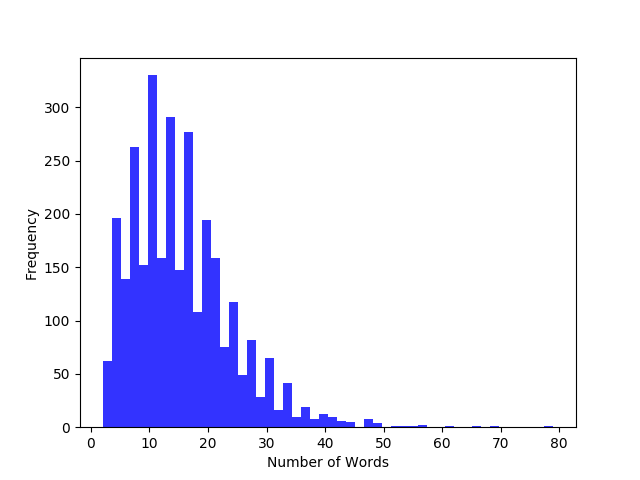
\includegraphics[width=0.6\textwidth, height=0.3\textwidth]{graphic/wordsnum_semval14_restaurants.png}\\
\\
\hline
名称 & 携程实体数据集\\
\hline
数据总数 & 6947条\\
语言 & 中文\\
词数最大值 & 100词数量级\\
90\%词数 & 20词数量级\\
情感分类准确度 & 较为正确\\
语句特点 & 语句较为规范,感情较为强烈\\
获取方式 & 对携程数据集进行过滤,取长度为10-100词之间,名词类词语只能为特定实体的语句进行手工标注实体和实体极性得到\\
主要用途 & 评估模型可行性及模型展示\\
词频统计 & 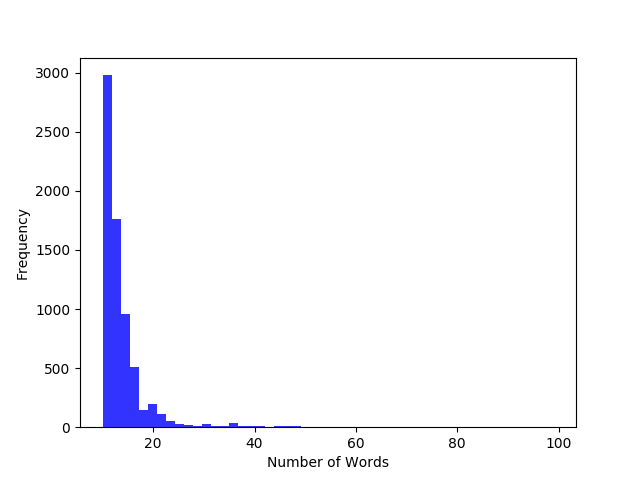
\includegraphics[width=0.6\textwidth, height=0.3\textwidth]{graphic/wordsnum_xiechengABSA.png}\\
\hline
\end{longtabu}  
\end{center}  

携程实体数据集所用到的实体如下:
\begin{itemize}
\item 地铁,整体,态度,服务员,性价比
\item 价格,前台,早餐,交通,位置
\item 设施,环境,房间,酒店
\end{itemize}
该实体集合是通过统计携程数据集上出现频率为前20的名词,经过人工筛选不规范的词汇后得到的。

\section{情感词典}
由于知识模型可以同时支持中/英文分析,故情感词典主要由以下两种语言共六个词典组成。
\subsection{中文情感词典}
\begin{enumerate}
\item Hownet(知网)情感词典\cite{hownet}:语言为中英双语,但本文主要使用中文部分。该词典为董振东和董强建立的情感分析用语集,包括主张词语,正面/负面情感词语,正面/负面评价词语,程度级别词语,并为程度级别词语划分强度等级,但其中有一些不符合构词法的词语,如“噲”,“媢”,“媢嫉”,“忺”,“安”,“巴”等在正面情感词典中出现的词。另外词语可能以短语形式出现,如“越...越...”,“abandon oneself to despaire”等。
\item NTUSD台湾大学情感词典:台湾大学自然语言处理实验室提供的情感词典,包括正面词汇2810个和负面词汇8276个,极性划分较为准确,且包含各种词性,如“一下子爆发”,“一下子爆发的一连串,“一巴掌”。
\item DUTIR情感词汇本体库:大连理工大学信息检索研究室整理和标注的中文情感词库,具有词性,情感分类,强度,极性和辅助情感分类,强度,极性等特征,划分详细。包含各种词性,但以成语和俗语为主体。
\end{enumerate}
\subsection{英文情感词典}
\begin{enumerate}
\item SentiWordNet\cite{sentiwordnet} \cite{sentiwordnet3}:基于WordNet3.0,具有语义,正向评分PosScore和负向评分NegScore等信息,本文中取PosScore-NegScore之差作为其分数。
\item Opinion Lexicon:Bing Liu等\cite{huliu2004a} \cite{huliu05a} 整理的极性情感词典,仅包含单词本身,不包含短语,但包括单词的各种变形形式。
\item 匹兹堡大学MPQA主观性词典\cite{mpqa}:是MPQA(Multi-Perspective Question Answering,多方面问答)系统所用到的词典,具有情绪词,词性,情感强弱等词汇信息。
\end{enumerate}

\section{数据预处理}
在有监督学习的过程中,如何选择特征,选择何种特征将对训练结果和泛化性产生极大的影响。实际环境中,文本往往含有不规范的表达方式及符号,需要对文本进行一系列处理。本文根据现有文献的经验,分析目前流行的文本预处理工具后,得出了下列文本预处理的流程。本文根据不同语言选择不同文本预处理工具,最终将中文或英文文本转化为可供模型分析的输入特征。

\subsection{基本流程}
如图\ref{preprocessing} 表示了整个文本情感分类系统的预处理流程,对所有模型,都需要对文本进行转换编码,去除非法字符,化繁为简和短句切分,分词这些预处理工作。其中分词则是重中之重,会对所有模型的准确率产生很大影响。对于机器模型,训练模式下需要生成词汇表,训练待编码特征对应的编码,并将语句各特征抽取出来以备训练或预测情感极性使用。
\begin{figure}[!hbp]
\begin{center}
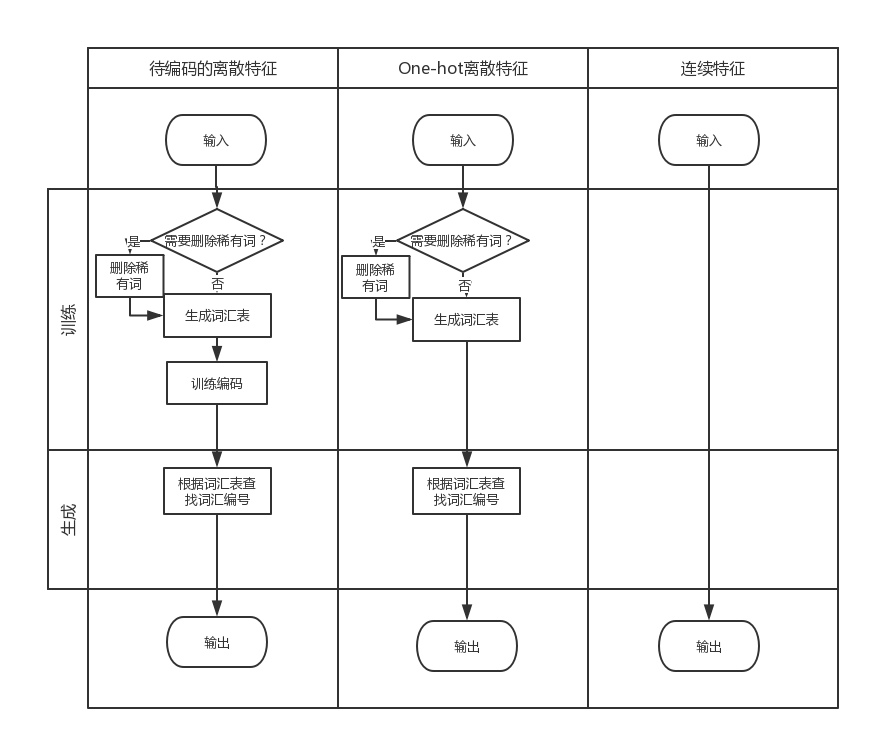
\includegraphics[width=\textwidth]{graphic/prepocessing.png}
\caption{数据预处理基本流程图 \label{preprocessing}}
\end{center}
\end{figure}

\subsection{分词和命名实体识别工具}
\subsubsection{中文}
本文分别从携程数据集,手机数据集和NLPCC中文任务中各随机抽取5条语句,使用相同的用户自定义词典,对比了三种分词工具:thulac,ansj,jieba的精准分词性能,结果如\nameref{appendix:parsercompare}所示。由于ansj工具的实体识别能力最强,故选择ansj工具。
ansj是由孙健实现的,具有分词,标注词性,实体识别,关键词抽取及新词发现功能的java中文分词工具。该工具使用隐马尔科夫模型进行语义消歧,使用Hash和高度优化Trie树进行词典匹配,并使用条件随机场模型(CRF)进行新词发现。\cite{ansjwiki} 本文主要使用到其分词,标注词性,实体识别及新词发现功能。\\
对于新词发现功能,本文主要学习输入语料中的新词,然后对这些新词进行手工过滤,加入情感词典以及ansj用户自定义词典。其中用户自定义词典人工过滤8430条,过滤得到3137条词条,157条情感词典词条。\\
\subsubsection{英文}
与没有分隔符的中文相比,英文短句中的单词之间由空格作为分隔符,更易于分隔,因而英文的分词难度远远小于中文分词。但由于英文文本中存在标点符号和不规则语用现象,本文选择使用Stanford CoreNLP工具进行分词。同时,这一步也是为了知识模型生成语法树做准备。\par
Stanford CoreNLP工具是由斯坦福大学自然语言处理实验室研发的\cite{corenlp},可以处理分句(ssplit),分词(tokenize),词性标注(POS),词干化(lemma),命名实体分析(NER),语法树分析(parse),短句情感分析(sentiment)和词语分析(natlog)等多种任务的工具集。本文中主要用到其中的分词,分句,词性标注,词干化,命名实体分析,语法树分析等功能。\par
该工具集基于Java,由管道(Pipeline)将各子工具连接,从而方便地复用了各子工具。\par
以下代码为本文系统JAVA部分调用Stanford CoreNLP工具的代码:\par
\lstset{language=java}
\begin{lstlisting}
new StanfordCoreNLP(
  PropertiesUtils.asProperties("annotators",
    "tokenize,ssplit,truecase,pos," + 
    "lemma,ner,parse,sentiment",
    "tokenize.language", "en"));
\end{lstlisting}

图\ref{fig:corenlpf1} \cite{corenlp} 是Stanford CoreNLP 整体流程的说明,如图,文本被转化为Annotation对象然后输入各子工具集,各子工具集可选,但内部存在依赖顺序。\par
表\ref{fig:corenlpf2} \cite{corenlp} 则是Stanford CoreNLP2014年各子工具集的语言支持情况,可以看到,该工具集可以处理多种语言,其中对英文支持最为全面准确。同时,该工具集支持中文的句法分析,满足知识模型需求。
\begin{center}
\begin{figure}
\subfigure[Stanford CoreNLP整体流程图]{
	\label{fig:corenlpf1}
	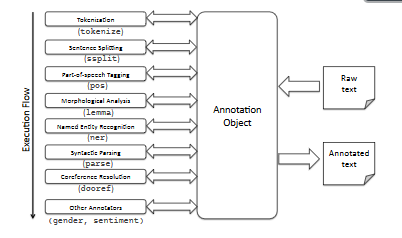
\includegraphics[width=0.4\textwidth]{graphic/stanfordcorenlpf1.PNG}
}
\subfigure[Stanford CoreNLP语言支持情况]{
	\label{fig:corenlpf2}
	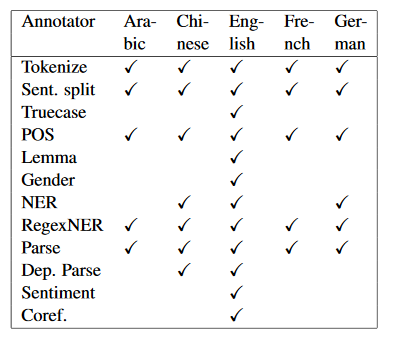
\includegraphics[width=0.4\textwidth]{graphic/stanfordcorenlpf2.PNG}
}
\end{figure}
\end{center}

\subsection{输入特征}
为了便于拓展模型和系统,本文将特征分为三类:
\begin{enumerate}
\item 待编码的离散特征,为了便于表示,称为Emb Feature。
\item One-hot离散特征: Onehot Feature。
\item 连续特征: D Feature。
\end{enumerate}
\par
三种特征各自有不同的处理方式。同时,对于某些离散特征,本文会删除词频较低的词汇,以提高模型拓展性,详细分析请见第三章。
\subsubsection{特征处理}
数据预处理方式见图\ref{featureprocessing},其中One-hot特征和Emb特征都需要转为编号,Emb特征需要进一步训练并转化为编码,生成阶段将Emb特征编号转化为编码与训练模型具体处理方式有关,因此本系统不将之列入预处理流程。
\begin{figure}[!hbp]
\begin{center}
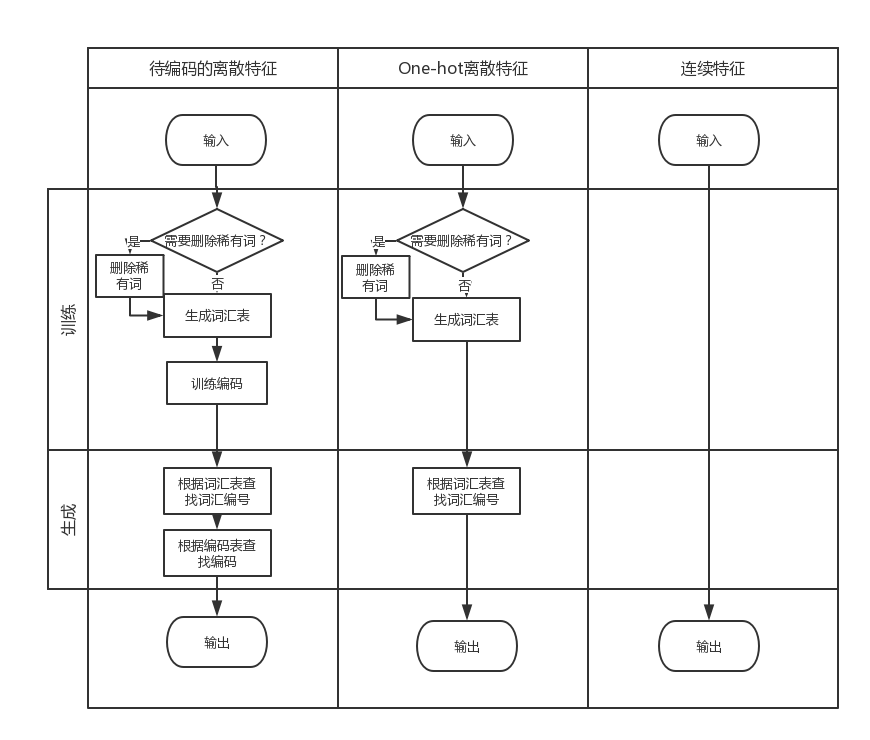
\includegraphics[width=\textwidth]{graphic/featurepocessing.png}
\caption{数据预处理基本流程图 \label{featureprocessing}}
\end{center}
\end{figure}
\subsubsection{特征选择}
\begin{center}
\begin{tabu}to \textwidth{X|X|X[3]|X[3]} 
\hline
& 层级 & 中文 & 英文\\
\hline
知识模型 & 语句级 & 词汇(D) & 词干化词汇(D)\\
\hline
CNN模型 & 语句级 & 词汇编号(Emb) & 词汇编号(Emb),词干编号(Emb)\\
\hline
RNN模型 & 语句级 & 词汇编号(Emb) & 词汇编号(Emb),词干编号(Emb)\\
\hline
CNN模型 & 实体级 & 词汇编号(Emb),词性编号(Onehot) & 词汇编号(Emb),词干编号(Emb),NER特征编号(Onehot)\\
\hline
RNN模型 & 实体级 & 词汇编号(Emb),词性编号(Onehot) & 词汇编号(Emb),词干编号(Emb),NER特征编号(Onehot)\\
\hline
\end{tabu}
\end{center}

\subsection{稀有词删除}
该步骤统计某特征的词频,对于词频小于规定次数的特征,将其置换为一个特殊词"RAREWORD"。对于词性为nt(机构团体), ns(地名), nr(人名), nz(其它专有名词)的单词所对应的特征,规定次数通常大于全局规定次数,以删除专有名词,尽量减少这类无用词的影响。

\subsection{英文词性还原及词干化}
英文中动词往往具有多种时态,如过去式,现在进行时,一般现在时等,如got,gotten,get,getting,gets。同时,形容词和副词也常常具有同样的词干,如happy, happily。这些单词虽然形态不同,却具有语义上的联系,因此,有必要对单词进行词性还原和词干提取,以发现其内部隐含的语义联系。\par
本文使用Stanford CoreNLP对单词进行词性还原,之后再使用nltk Snowball Stemmer进行词干化,以此作为英文模型的输入特征。相关测试见\nameref{appendix:lemmacompare}。